% ==================================================
% 4.5 住宅場景整合任務
% ==================================================
\section{住宅場景整合任務}
\label{sec:residential_integrated_task}

住宅任務將導航、視覺定位與機構操作串接於同一流程，
檢查控制器能否由不同感知目標與任務階段持續產生全身命令。
本節先以同一次含四名行人的完成案例，
說明開門、圓柱取物、抽屜取筆、收納及回程關門的執行結果，
再彙整無行人與含行人條件下的完成情形及策略比較。
持物與機構操作沿用第 3.6 節的固定相對位姿假設，
結果用於評估運動與任務銜接；摩擦抓持及滑移的適用範圍於第 4.6 節討論。

% ==================================================
% 4.5.1 視覺導引之開門與穿門
% ==================================================
\subsection{視覺導引之開門與穿門}
\label{subsec:residential_visual_door_passage}

機器人由臥室起點出發，先取得門把與門扇觀測，
再由時間對齊後的幾何量建立抓取位姿與底盤接近參考。
視覺前端使用機身與手腕相機的 RGB-D 資料，
RGB 影像進入實例分割，深度則用於目標幾何估測。
\cref{fig:ch4_residential_visual_observations}呈現同一案例在不同階段的目標影像。
門把、圓柱、抽屜把手與筆狀物件具有不同形狀及觀測距離，
各目標依第 3.5 節的幾何程序轉換為操作參考。

\begin{figure}[htbp]
    \centering
    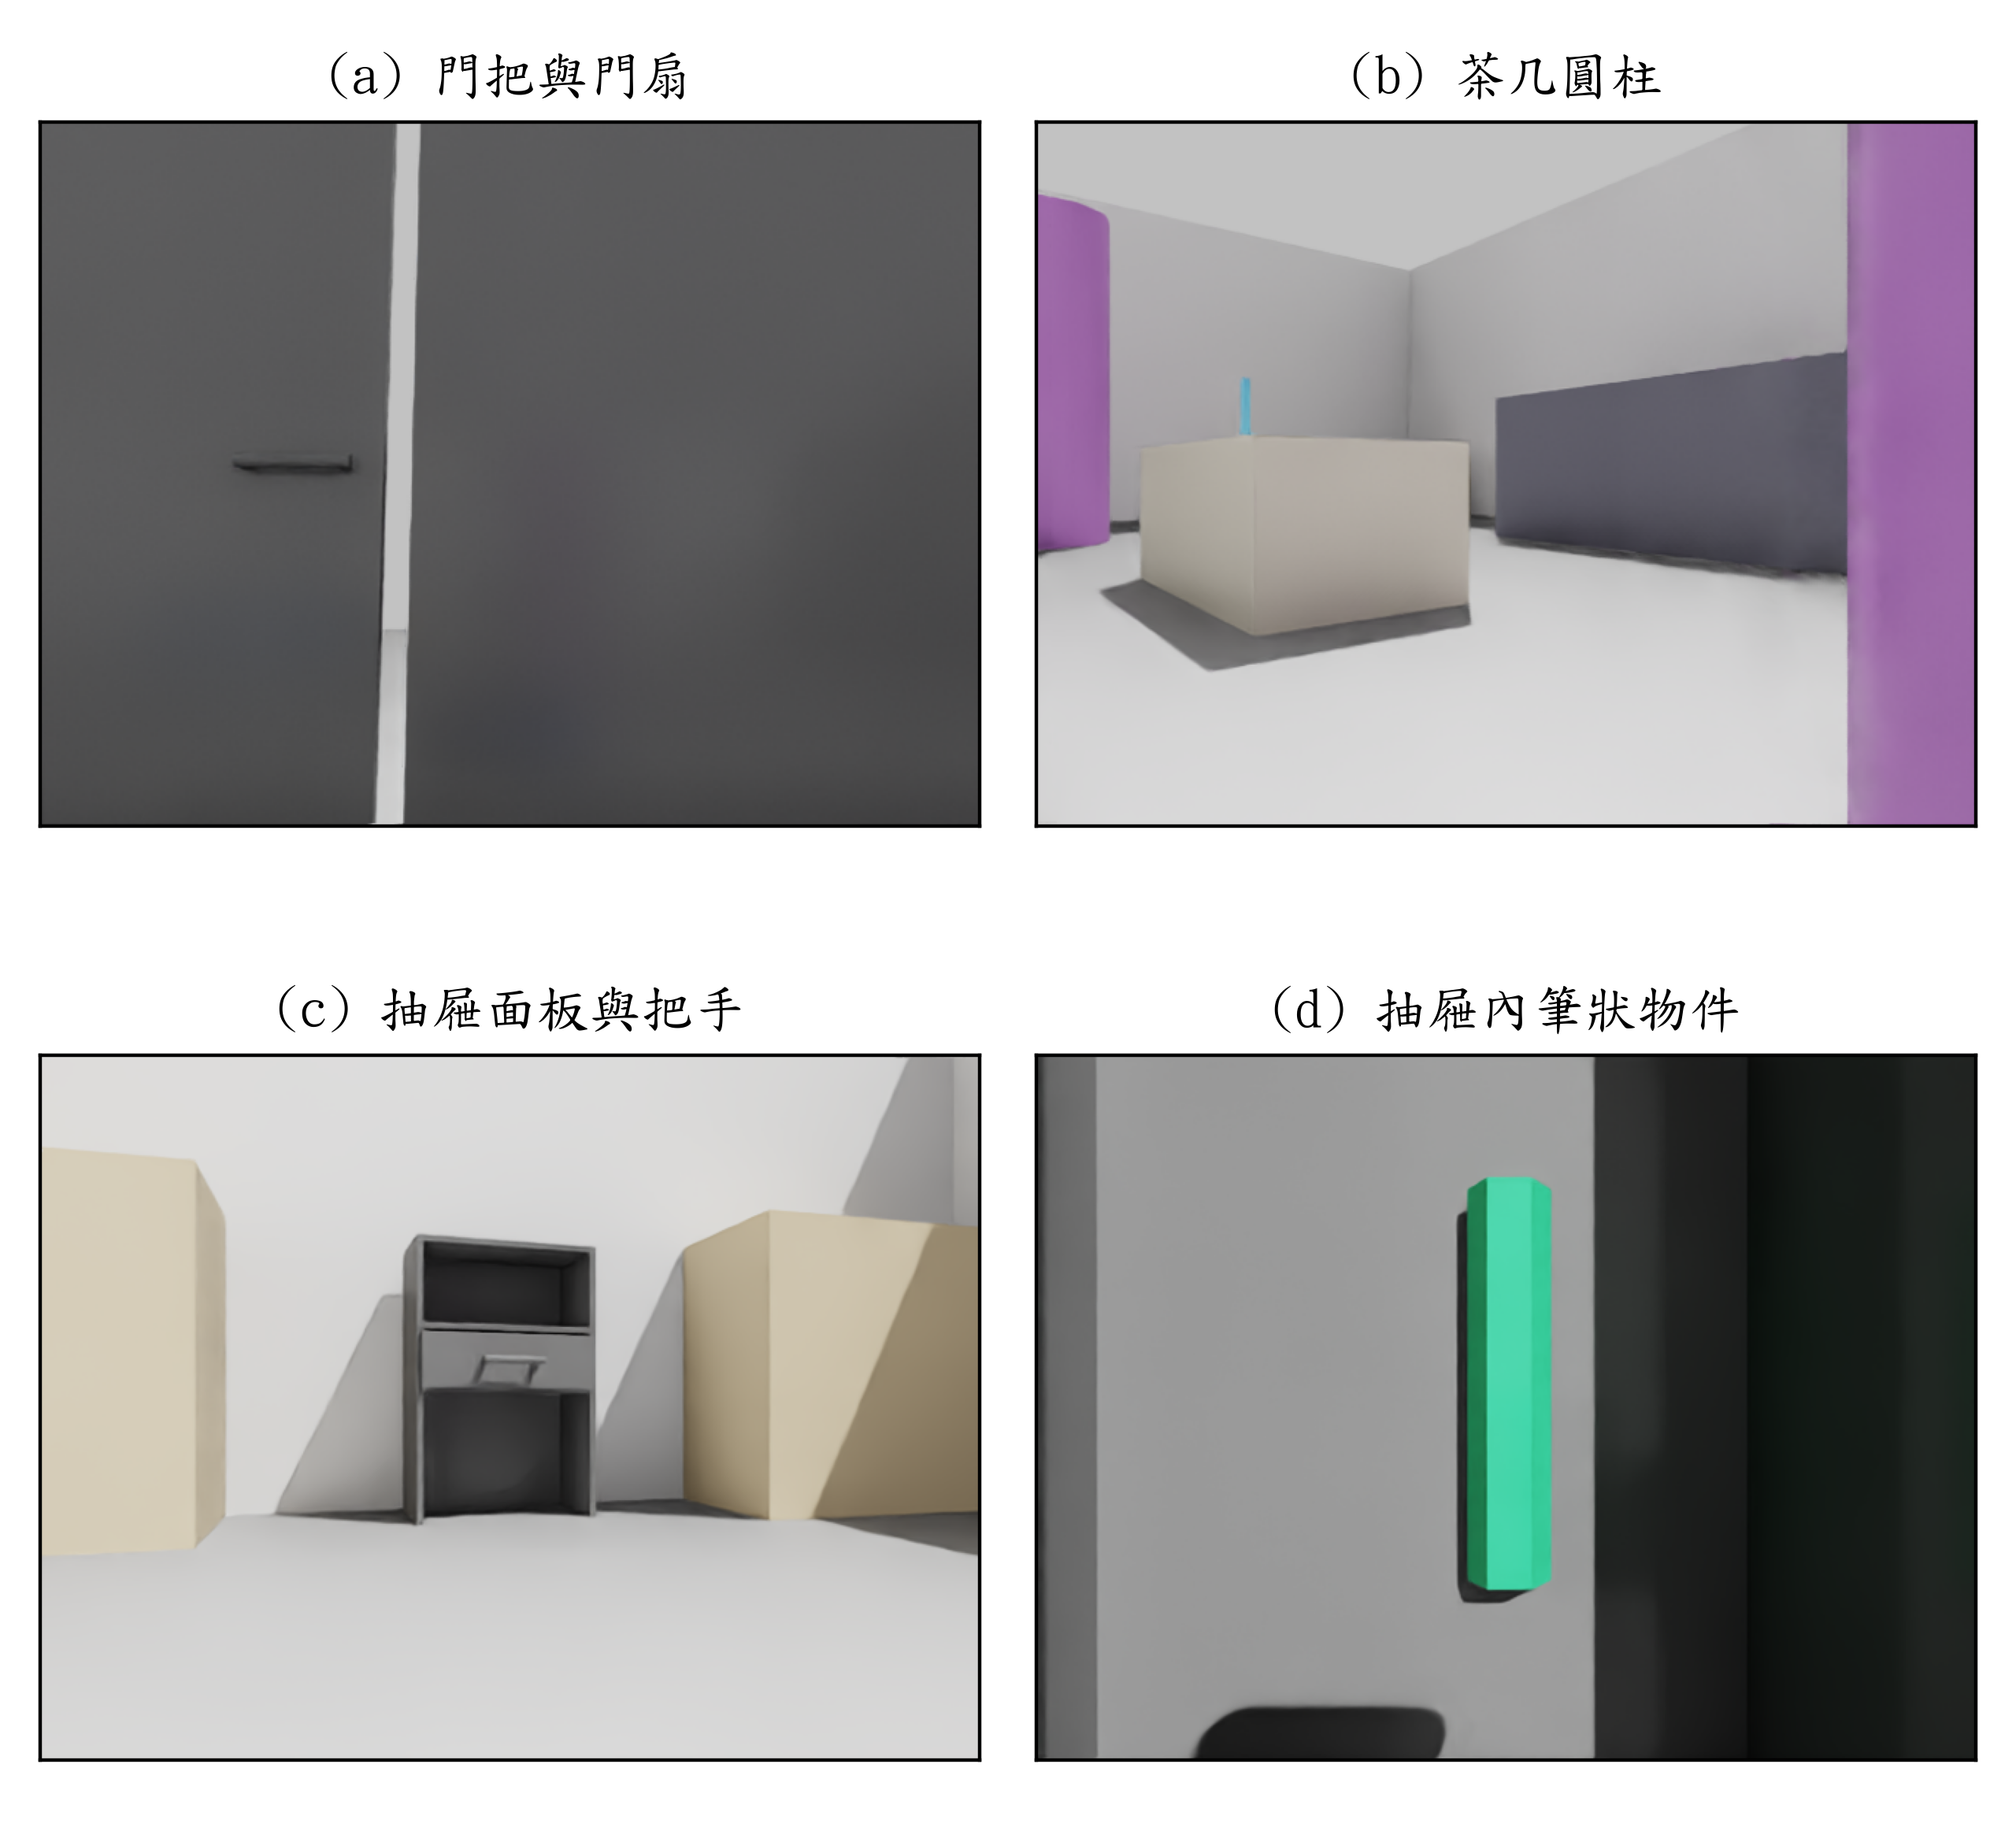
\includegraphics[width=0.98\textwidth]{figsrc/ch04/residential_visual_observations.png}
    \caption{住宅任務之 RGB 目標觀測：
    (a) 門把與門扇；(b) 茶几圓柱；
    (c) 抽屜面板與把手；(d) 抽屜內筆狀物件。
    (a)、(d) 為手腕相機影像，(b)、(c) 為機身相機影像。}
    \label{fig:ch4_residential_visual_observations}
\end{figure}

在此案例由控制接手至門把接近開始前的區間內，
共取得 $27$ 筆有效門把位置觀測。
以模擬幾何作離線對照，位置誤差中位數為 $1.41$ mm，
最大值為 $4.36$ mm。
這項統計對應該區間的有效幾何估測，
與影像分割準確度及後續末端追蹤誤差分別評估。
目標通過有效性與時間條件後，
底盤依導航參考接近，手臂同步展開並於末段併入世界座標抓取線。

抓持建立後，門角參考沿鉸鏈模型推進，
底盤與手臂共同配合把手的圓弧運動。
\cref{fig:ch4_residential_door_open_close}(a)顯示，
由控制接手至開門完成約需 $27.50$ s，門角達約 $85.02^\circ$。
解除抓持並確認手指張開後，
末端先退出門把，再銜接收臂與穿門導航。
此交接依實際執行回報推進，
使機器人在離開把手後才承接後續通行動作。

\begin{figure}[htbp]
    \centering
    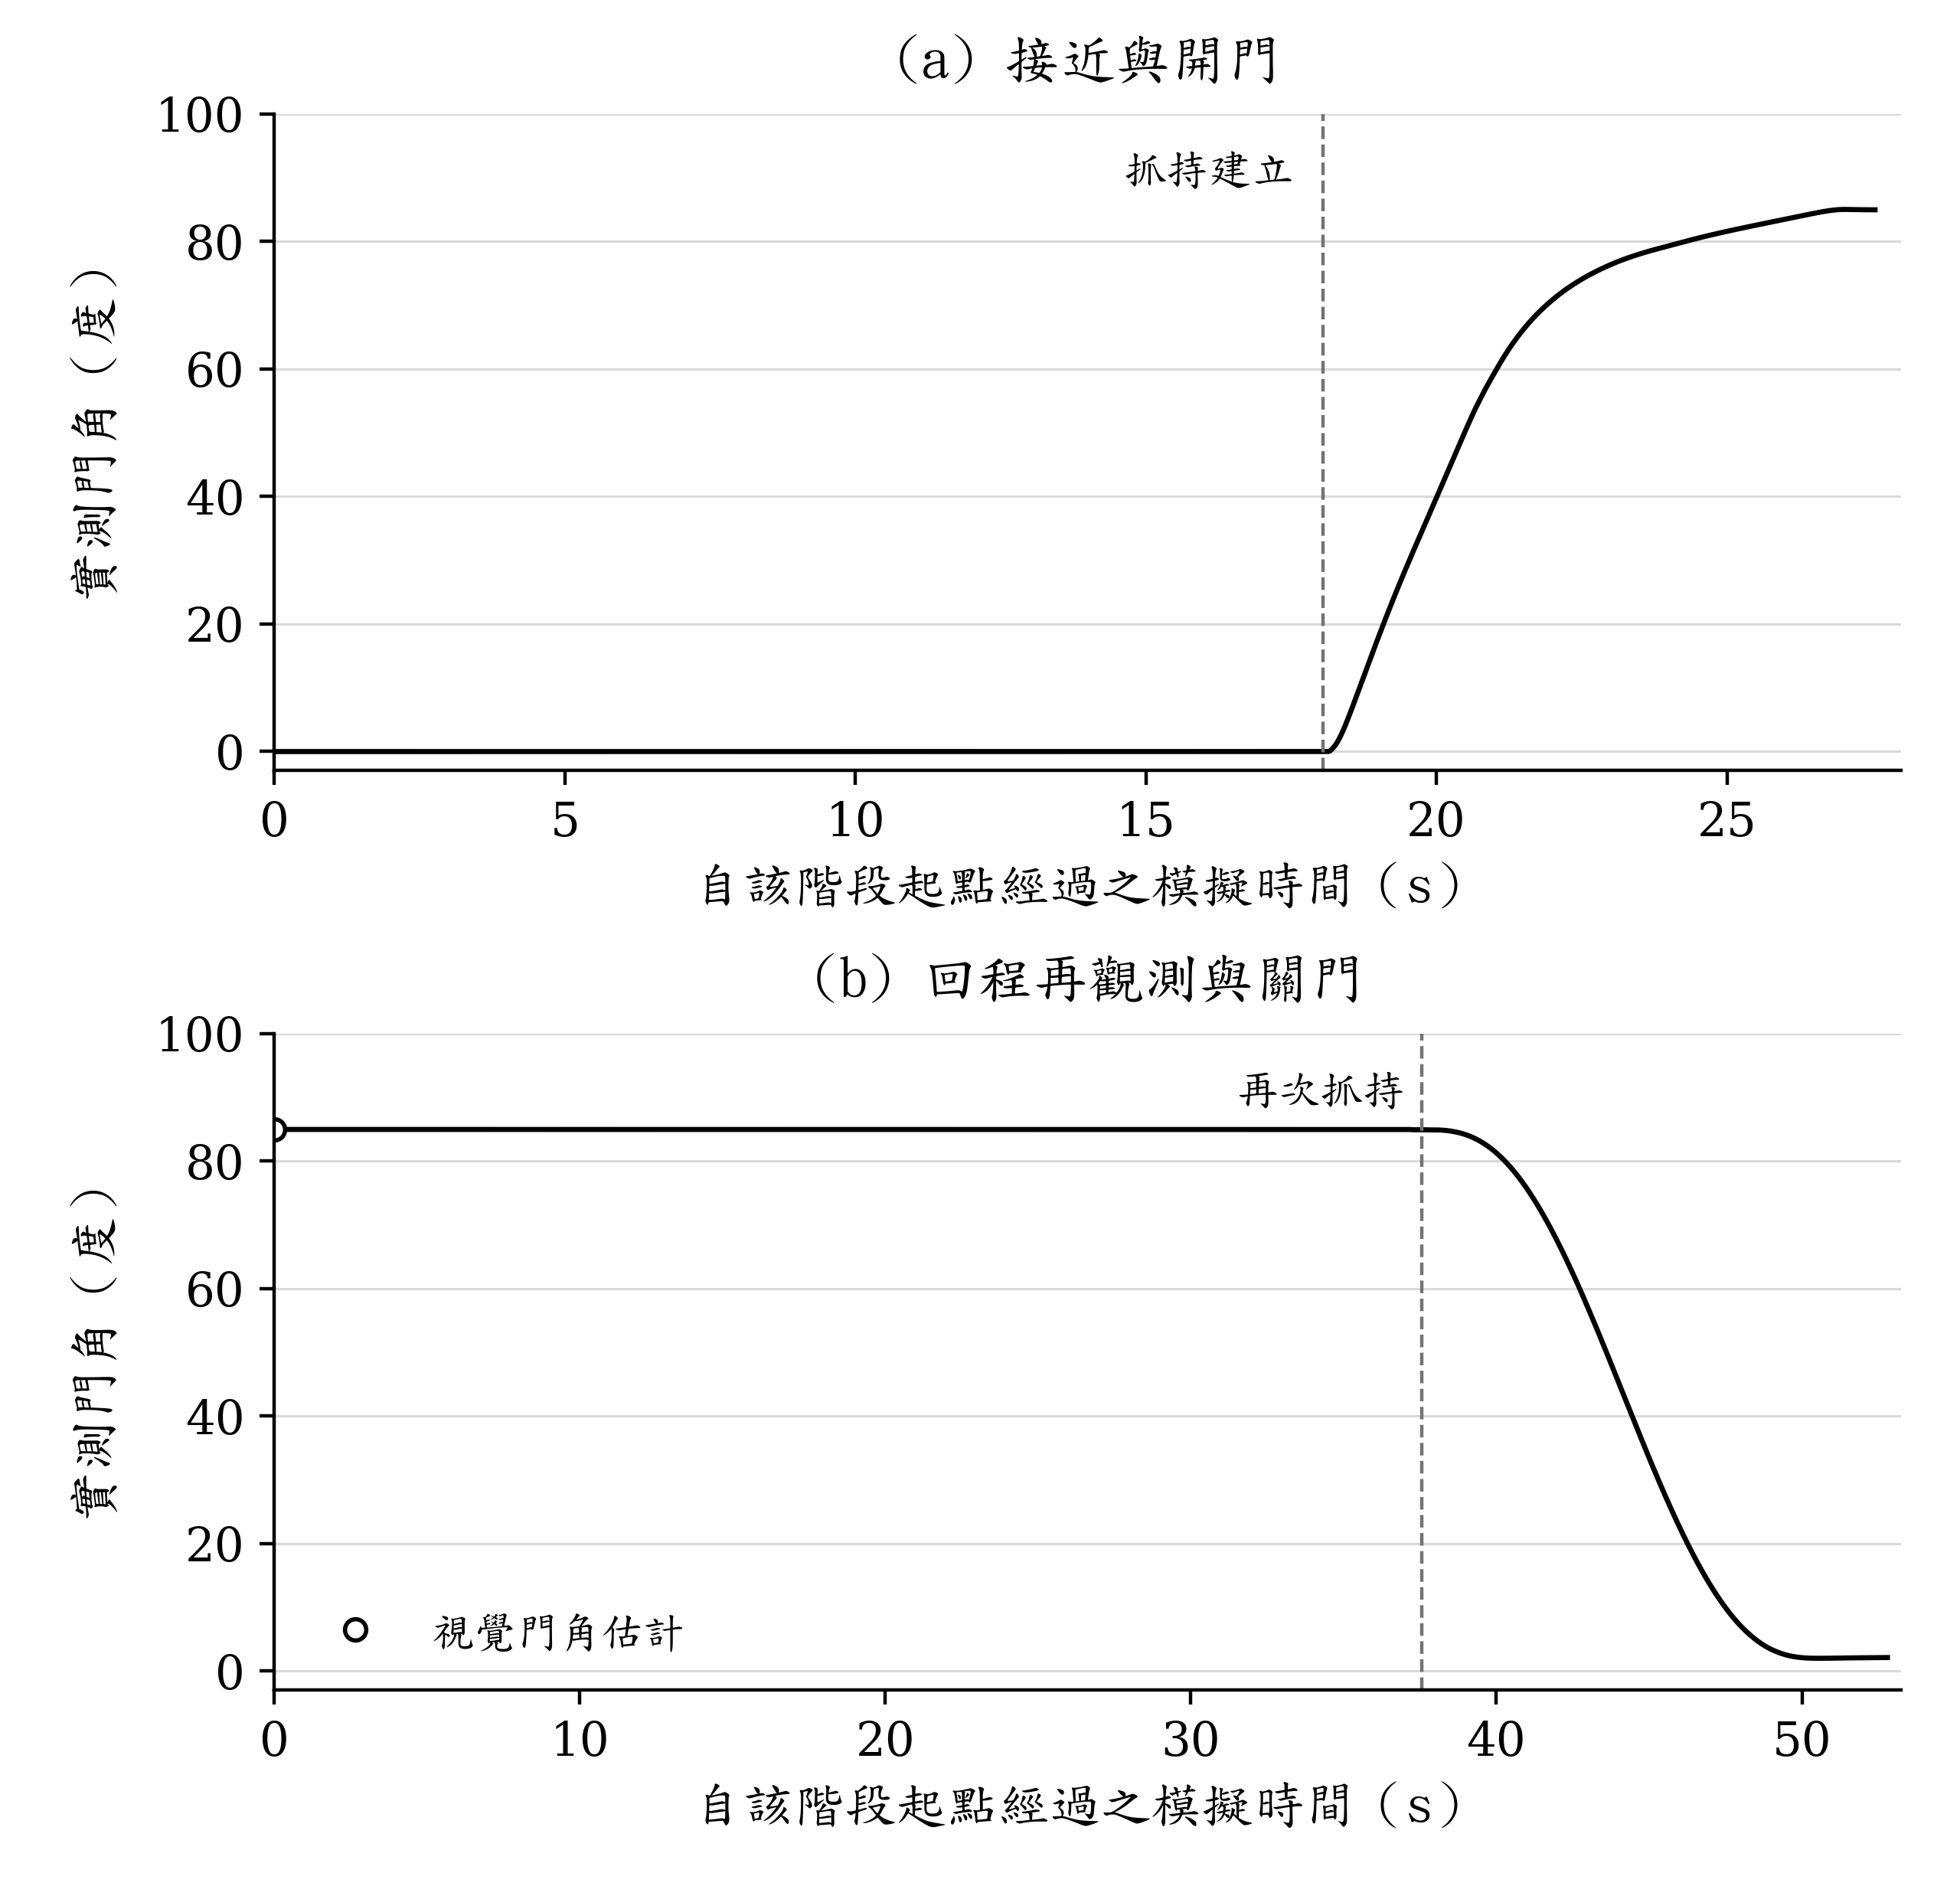
\includegraphics[width=0.98\textwidth]{figsrc/ch04/residential_door_open_close.png}
    \caption{同一次住宅任務之門扇操作：
    (a) 由控制接手至開門完成的實測門角；
    (b) 回程視覺再觀測至關門完成的實測門角。
    兩圖各由其階段起點計時，虛線標示抓持建立時刻；
    (b) 的空心圓為回程視覺門角估計。}
    \label{fig:ch4_residential_door_open_close}
\end{figure}

% ==================================================
% 4.5.2 茶几圓柱之移動中抓取與車尾收納
% ==================================================
\subsection{茶几圓柱之移動中抓取與車尾收納}
\label{subsec:residential_mobile_cylinder_storage}

通過門口後，機器人前往客廳茶几，
以圓柱觀測建立目標位置，再選擇具有導航可達性與連續手臂構型的操作區域。
本案例圓柱半徑為 $15$ mm、高度為 $200$ mm，
初始位置位於茶几側邊。
底盤接近時，手臂先依構型參考展開，
後段逐步轉為追蹤世界固定的抓取位置，
使底盤推進與末端接近在同一控制流程中重疊。

\cref{fig:ch4_residential_cylinder_mobile_pick}(a)呈現接近至收納期間的底盤速率。
由閉爪開始至抓持確認約為 $0.95$ s，
底盤累積移動約 $53.2$ mm，平均平移速率約為 $0.056$ m/s。
因此，此案例的閉爪與確認發生於底盤仍在移動的期間。
閉爪開始時，末端對操作參考的位置與姿態誤差分別約為 $4.45$ mm 與 $0.72^\circ$，
用於描述抓取銜接時的追蹤狀態。

\begin{figure}[htbp]
    \centering
    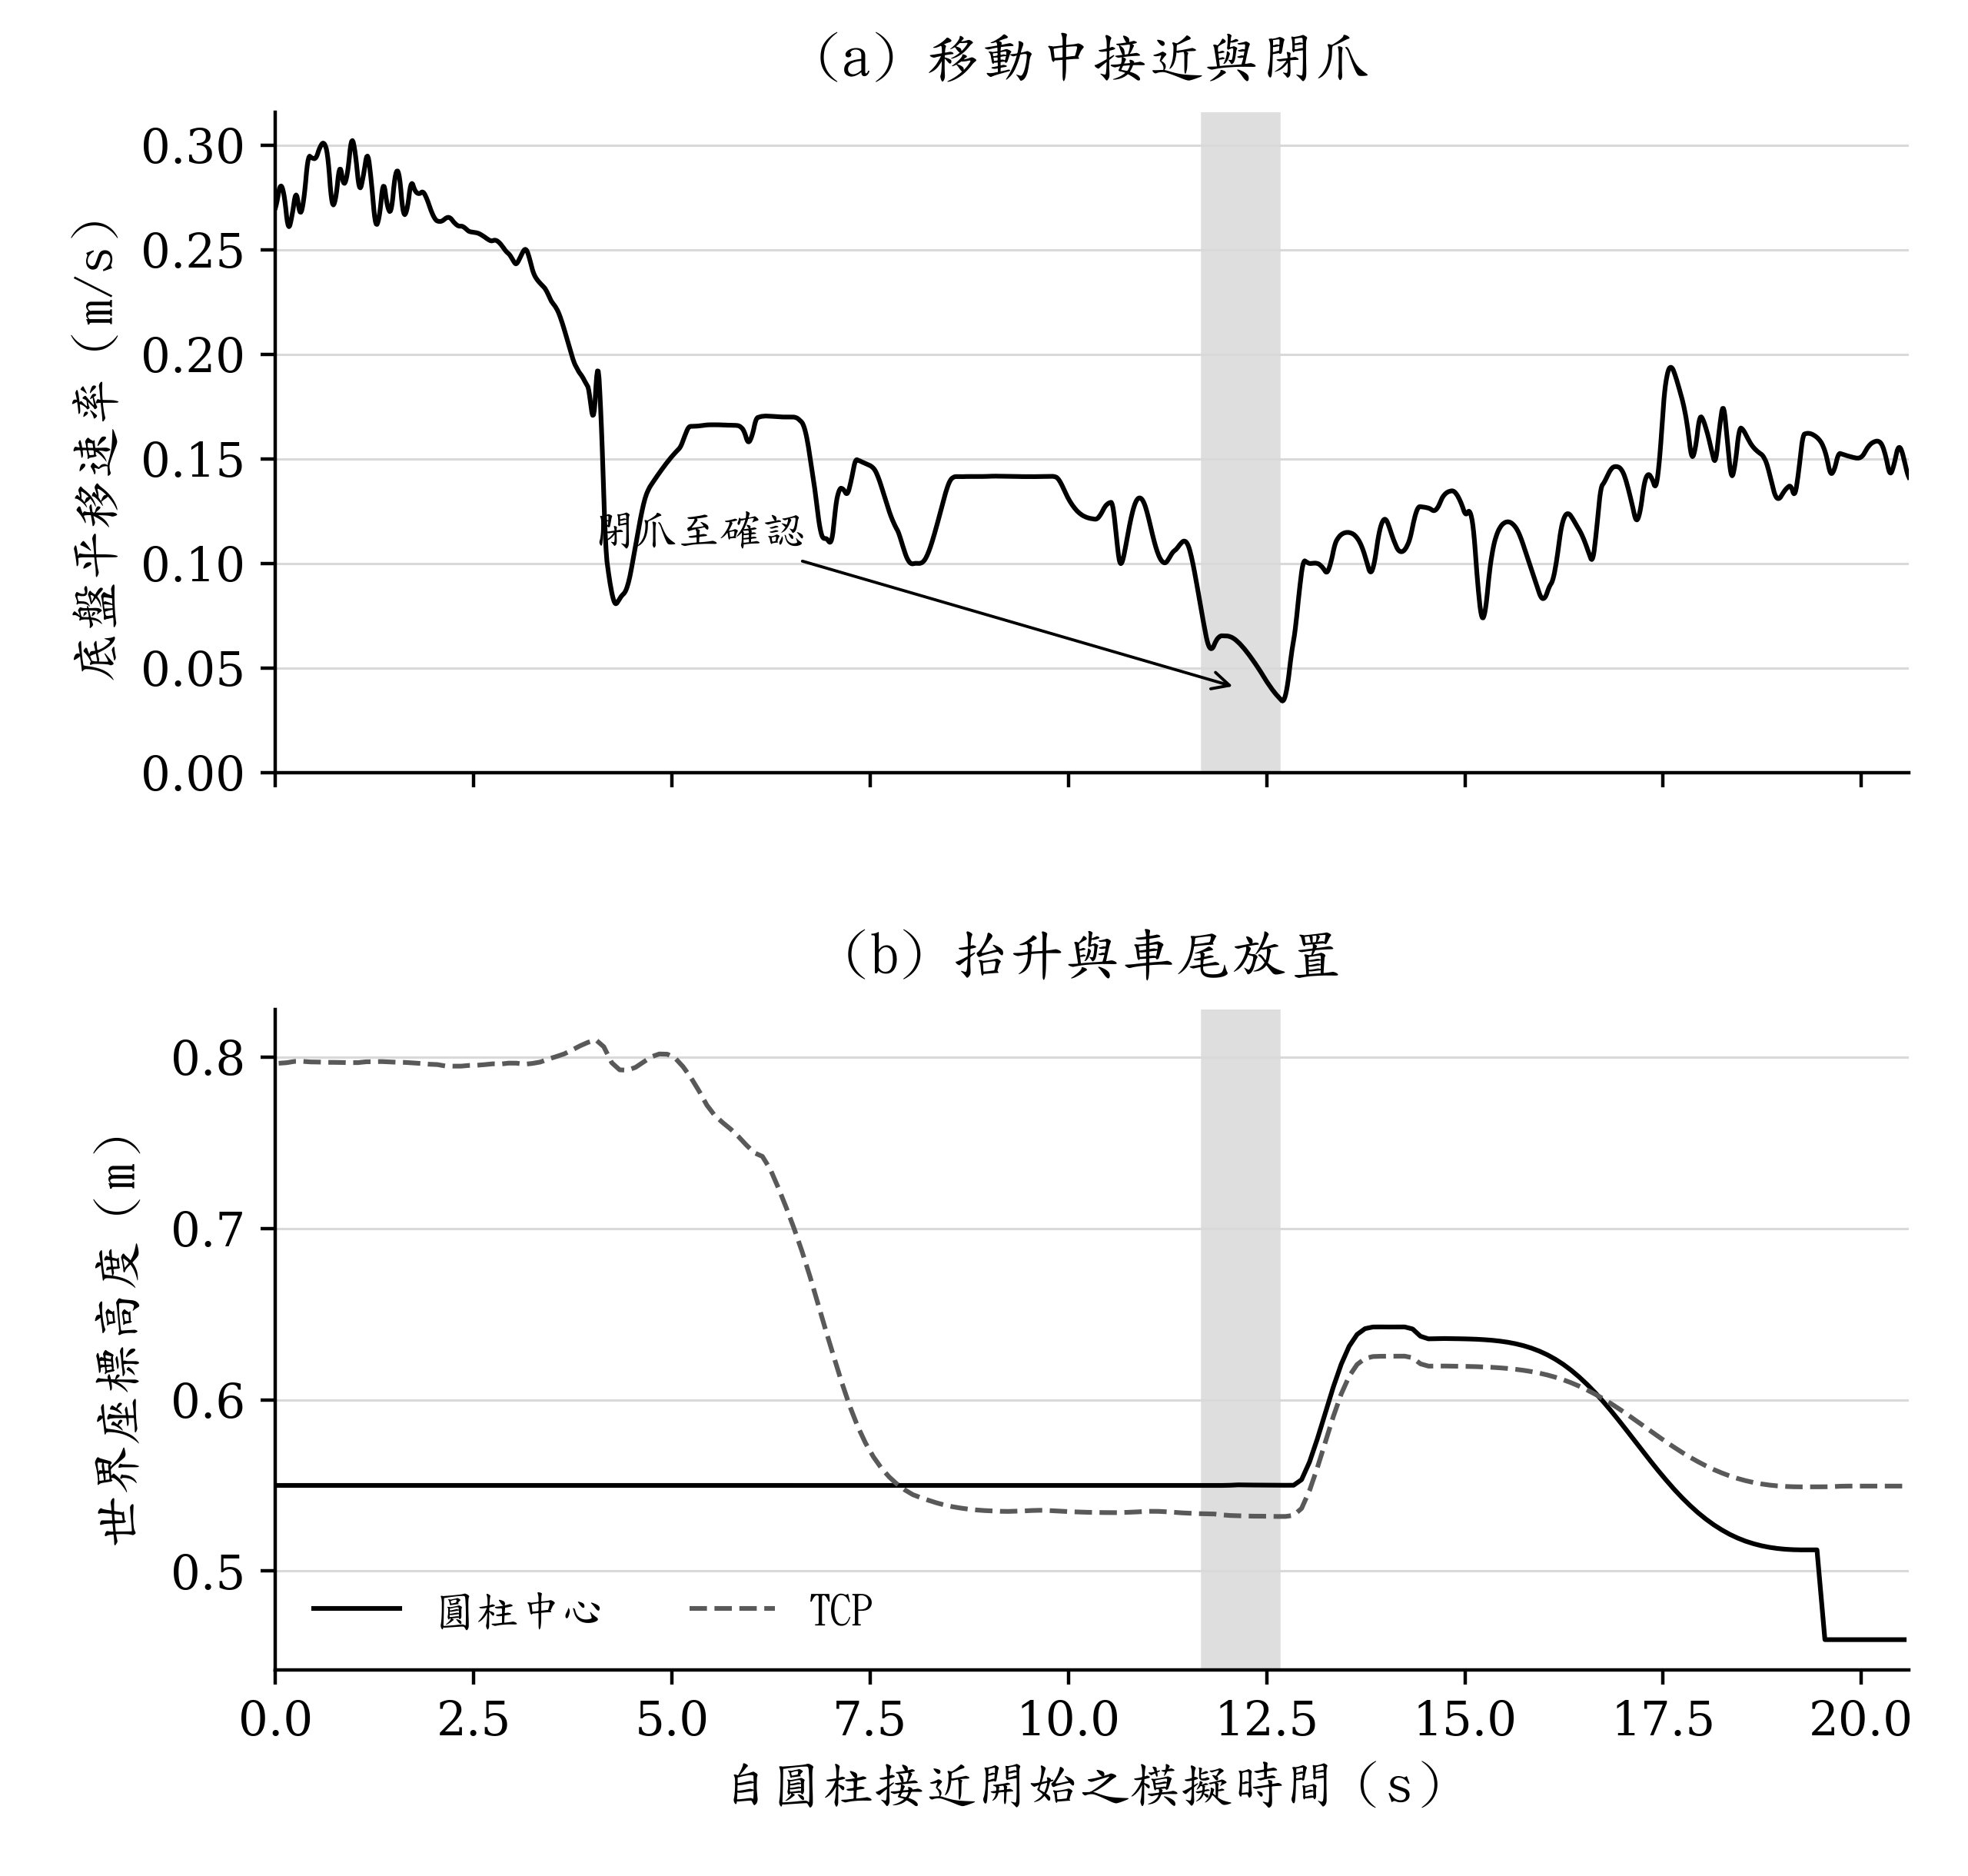
\includegraphics[width=0.98\textwidth]{figsrc/ch04/residential_cylinder_mobile_pick.png}
    \caption{住宅案例之圓柱移動中抓取與收納：
    (a) 底盤平移速率，以 $0.10$ s 位置差分計算；
    (b) 圓柱中心與 TCP 的世界座標高度。
    灰色區間為閉爪開始至抓持確認，兩圖使用相同時間基準。}
    \label{fig:ch4_residential_cylinder_mobile_pick}
\end{figure}

抓持確認後，末端參考轉為底盤相對目標，
接續抬升、移向車尾盒上方、釋放與收臂。
\cref{fig:ch4_residential_cylinder_mobile_pick}(b)顯示物件隨抬升離開桌面，
再於車尾放置階段降低高度。
放置時先完成解除抓持的執行確認，再張爪並等待物件落下，
後續由實際構型建立收臂參考。
任務結束時另以物件中心在盒體座標中的位置核對收納結果，
避免僅由放置階段事件推定物件已留在盒內。

% ==================================================
% 4.5.3 開抽屜取筆、收納與關閉抽屜
% ==================================================
\subsection{開抽屜取筆、收納與關閉抽屜}
\label{subsec:residential_drawer_marker_storage}

圓柱收納後，機器人前往右側房間的抽屜櫃。
家具登錄位置提供搜尋先驗，當次面板與把手觀測則用於修正操作幾何。
此案例的實際抽屜位置相對登錄位置偏移約 $44.7$ mm，
朝向差為 $2^\circ$；融合五筆觀測後，
所估櫃體平面位置與模擬幾何的差約為 $7.8$ mm。
控制端依更新後的滑軌方向建立接近、拉開及後續選位參考。

抓住把手後，抽屜沿滑軌拉出至約 $200$ mm。
\cref{fig:ch4_residential_drawer_pick_close}(a)顯示完整開度歷程，
(b)則比較拉開期間的底盤軸向平移與抽屜開度變化。
兩者具有相近的位移趨勢，
表示底盤移動承接此階段主要的滑軌方向運動，
手臂持續配合末端位姿與構型需求。
拉開結束且解除抓持時，控制端估計開度為 $200.50$ mm，
對應的模擬實測開度為 $200.29$ mm。

\begin{figure}[htbp]
    \centering
    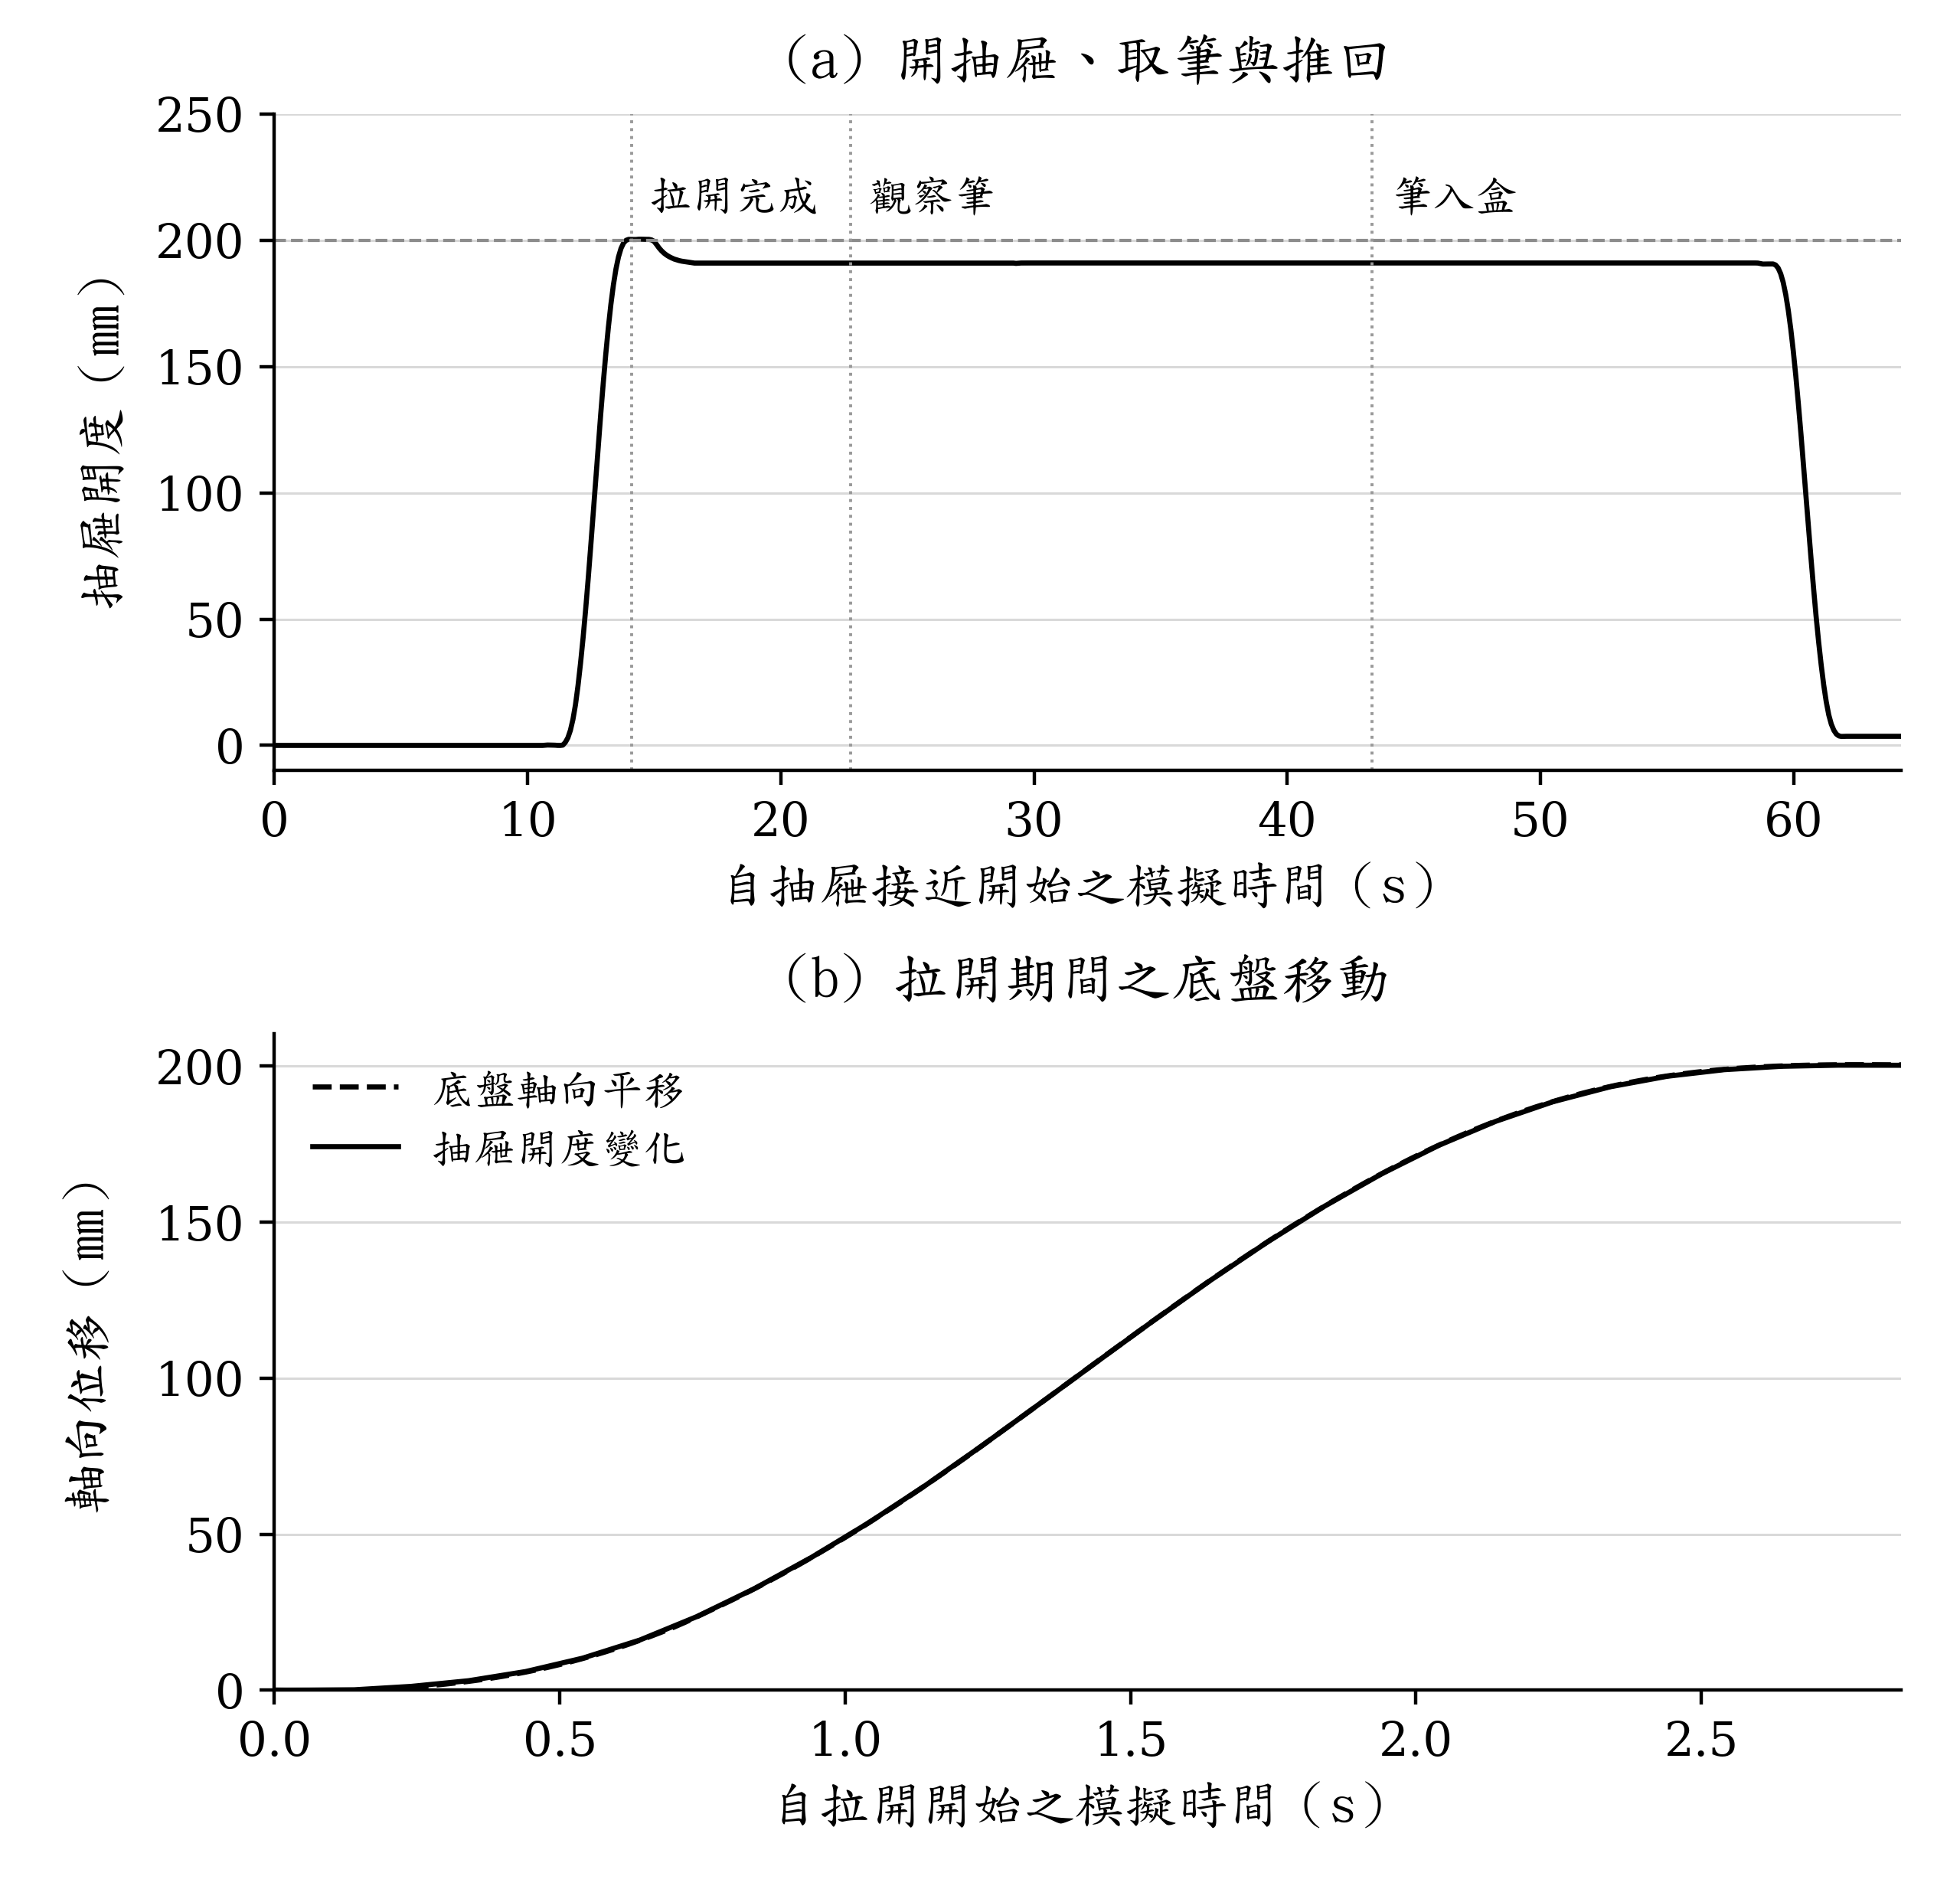
\includegraphics[width=0.98\textwidth]{figsrc/ch04/residential_drawer_pick_close.png}
    \caption{住宅案例之抽屜操作：
    (a) 自把手接近開始至關抽屜完成的實測開度，水平虛線為 $200$ mm；
    (b) 拉開期間的底盤軸向平移與抽屜開度變化。
    (a) 的垂直點線標示拉開完成、觀察筆與筆入盒事件，
    (b) 的位移由拉開起點計算。}
    \label{fig:ch4_residential_drawer_pick_close}
\end{figure}

解除把手抓持後，手臂轉至抽屜上方的觀察構型，
再由筆狀物件的遮罩、深度與主軸估測建立抓取位姿。
本實驗使用長度約 $140$ mm 的粗筆狀代理物，
抓取方向依主軸與可行手臂構型選擇。
完成接近與抬升後，先退出抽屜附近空間，
再銜接車尾收納及收臂。
以圓柱入盒事件至筆入盒事件計算，
此區間共需 $75.60$ s，涵蓋兩操作區之間的導航、
把手定位、開抽屜、觀察、取筆與放置。

關抽屜前重新觀測把手，依更新位置修正推回起點，
再由相同滑軌方向建立反向運動參考。
推回結束且解除抓持時，控制端估計剩餘開度約為 $4.74$ mm，
模擬實測值約為 $3.58$ mm；整體任務結束時為 $3.61$ mm。
推回參考在關閉端預留 $5$ mm 行程，
因此本案例以接近關閉位置作為終點，保留與機構硬限位之間的餘量。

% ==================================================
% 4.5.4 回程通行、關門與返回起點
% ==================================================
\subsection{回程通行、關門與返回起點}
\label{subsec:residential_return_door_closing}

完成關抽屜後，機器人沿導航路徑返回門口。
本案例回程時門扇仍維持約 $85^\circ$，
先由視覺再觀測門角，通過既有開口後，再接近臥室側的把手操作位置。
回程視覺門角估計為 $84.876^\circ$，
同一觀測時刻的模擬實測值約為 $84.932^\circ$，差約 $0.056^\circ$。
新的把手目標由該門角與鉸鏈幾何重建，
使回程接近能對應當時的門扇狀態。

再次抓持後，底盤與手臂依繞鉸鏈的共轉參考執行關門。
\cref{fig:ch4_residential_door_open_close}(b)顯示，
抓持前門角維持穩定，操作開始後逐步減少至約 $2^\circ$。
解除抓持時的實測門角約為 $1.99^\circ$，
完成張爪與末端退出後約為 $2.11^\circ$。
此階段結束後，機器人收臂並返回起點，
終點與起始位置的平面距離約為 $0.134$ m，
符合本組整合任務所使用的 $0.60$ m 返回範圍。

\cref{tab:ch4_residential_terminal_states}整理代表案例的終態。
圓柱與筆狀物件均位於收納判定範圍，
抽屜與門扇停在所設定的近關閉位置，
底盤亦返回起點附近。
物件入盒判定使用其中心位置，
門角與抽屜開度則由模擬機構狀態另行核對。
表中物件位置以收納盒所屬之 \texttt{base\_link} 座標表示。

\begin{table}[htbp]
    \centering
    \caption{住宅代表案例之任務終態核對}
    \label{tab:ch4_residential_terminal_states}
    \begingroup
    \small
    \renewcommand{\arraystretch}{1.25}
    \begin{tabular}{p{0.21\textwidth} p{0.40\textwidth} p{0.25\textwidth}}
        \hline
        項目 & 任務結束時之量測 & 核對內容 \\
        \hline
        圓柱中心 & $(-0.140,\ 0.024,\ 0.301)$ m & 位於收納範圍 \\
        筆狀物件中心 & $(-0.095,\ 0.039,\ 0.299)$ m & 位於收納範圍 \\
        抽屜剩餘開度 & $3.61$ mm & 接近關閉位置 \\
        門扇角度 & $2.17^\circ$ & 接近 $2^\circ$ 參考 \\
        底盤返回距離 & $0.134$ m & 小於 $0.60$ m \\
        \hline
    \end{tabular}
    \endgroup
\end{table}

% ==================================================
% 4.5.5 任務銜接與整體完成情形
% ==================================================
\subsection{任務銜接與整體完成情形}
\label{subsec:residential_task_completion}

\cref{fig:ch4_residential_mission_timeline}將上述操作放回同一任務的底盤軌跡與時間軸。
由控制接手至返回完成共需約 $335.3$ s，皆以模擬時間計算，
交權前的起動準備另行保留。
依開門完成、圓柱入盒、筆入盒、關抽屜、關門與返回等事件切分，
六段時間依序約為 $27.5$、$71.1$、$75.6$、$20.9$、$110.7$ 與 $29.5$ s。
各段包含相應的導航、操作與等待，
因此其長度同時反映路線、觀測及階段銜接的影響。

\begin{figure}[htbp]
    \centering
    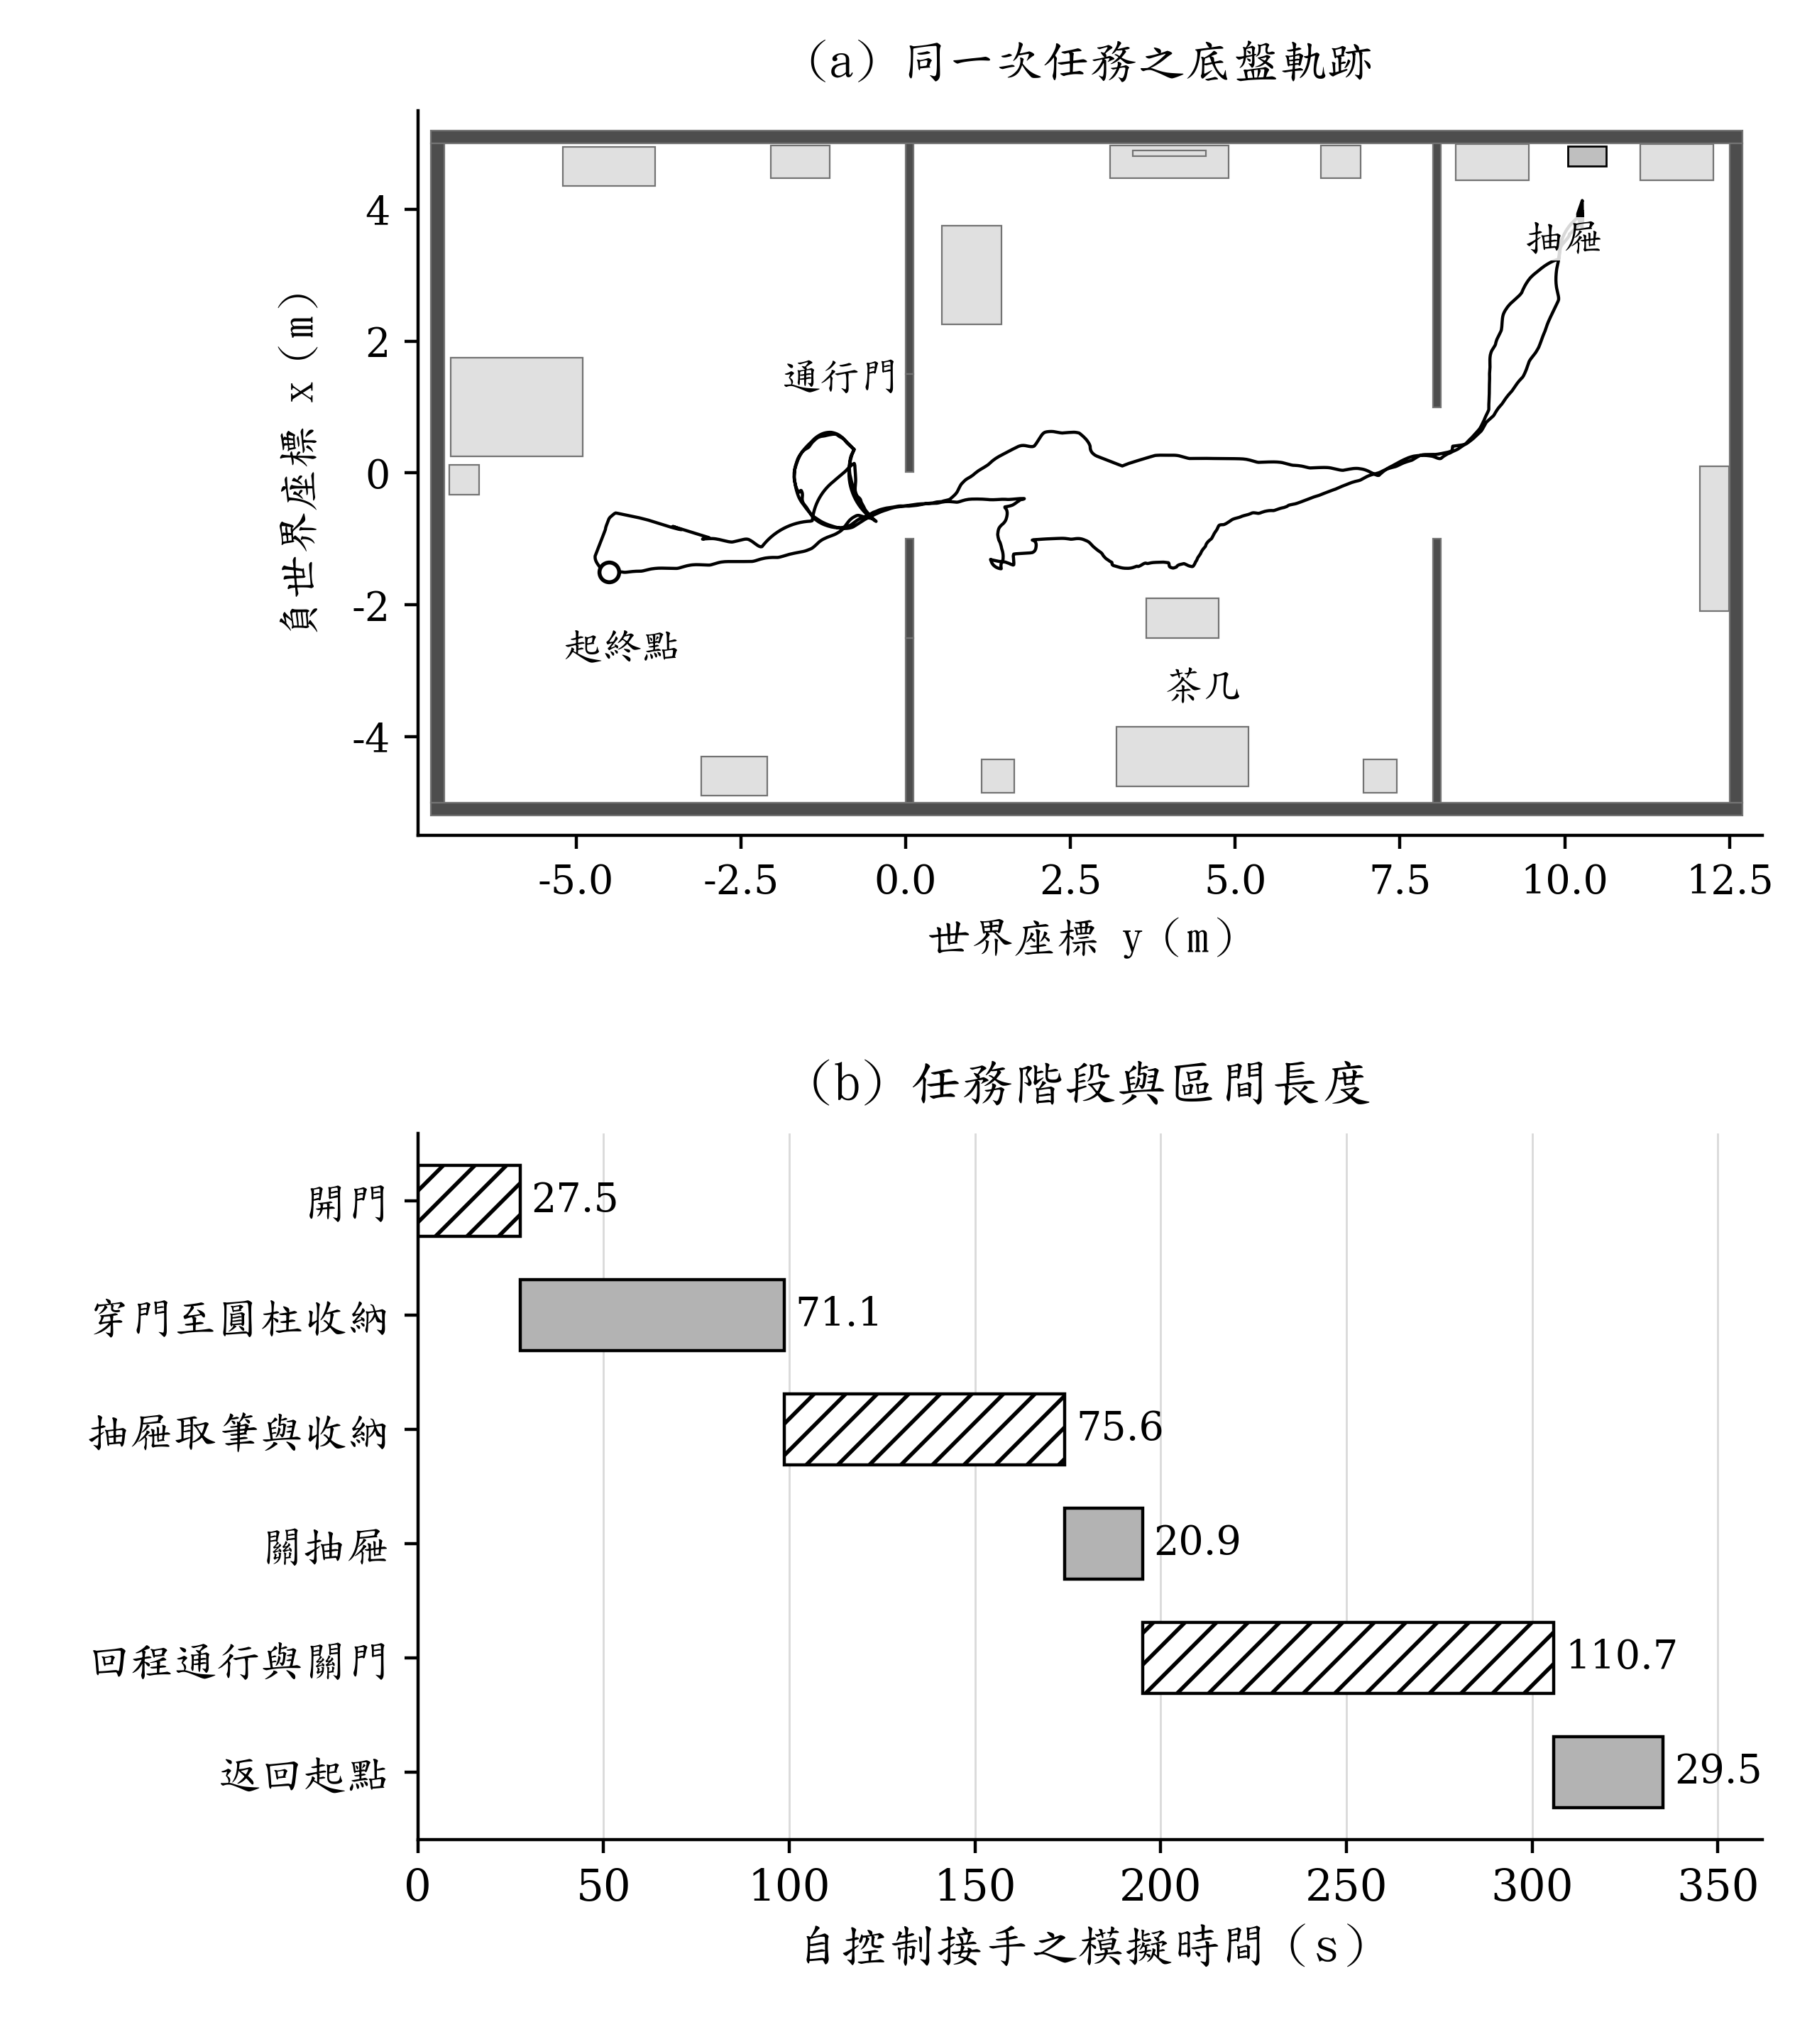
\includegraphics[width=0.98\textwidth]{figsrc/ch04/residential_mission_trajectory_timeline.png}
    \caption{同一次住宅整合任務之運動與階段銜接：
    (a) 底盤軌跡與固定場景底圖，空心圓為起點；
    (b) 由控制接手起算的任務時間軸，條形旁數值為各區間長度，單位為秒。}
    \label{fig:ch4_residential_mission_timeline}
\end{figure}

除代表案例外，另彙整 $43$ 次住宅整合紀錄，
其中無行人條件為 $27$ 次，含行人條件為 $16$ 次。
含行人場景配置四名移動物件，
並保留其接近機器人時的暫停讓行規則。
\cref{tab:ch4_residential_completion_counts}列出完成與未完成數。
完成判定要求具有回程關門及兩次收納事件，
底盤終點位於返回範圍；完成案例另核對兩物件的終態收納位置。
這批紀錄包含整合期間的控制與交接修正，
完成數用於描述所測流程，不作為固定版本的成功率估計。

\begin{table}[htbp]
    \centering
    \caption{住宅整合紀錄之完成情形}
    \label{tab:ch4_residential_completion_counts}
    \begingroup
    \small
    \renewcommand{\arraystretch}{1.25}
    \begin{tabular}{l l c c c}
        \hline
        環境條件 & 接近策略 & 紀錄數 & 完成數 & 未完成數 \\
        \hline
        無行人 & 移動中操作 & $15$ & $9$ & $6$ \\
        無行人 & 停駐後操作 & $12$ & $9$ & $3$ \\
        含行人 & 移動中操作 & $8$ & $4$ & $4$ \\
        含行人 & 停駐後操作 & $8$ & $7$ & $1$ \\
        \hline
    \end{tabular}
    \endgroup
\end{table}

策略時間比較採用無行人條件下，兩種策略皆有完成案例的八個圓柱位置種子。
住宅停駐策略先完成接近前的停車，再展臂與接近；
後續機構操作仍允許全身協同運動，
與第 4.4 節的全區間底盤保持對照分別解讀。
同一種子與策略若有重複完成紀錄，先取其平均，
再對八個種子等權平均，以避免重複次數影響整體權重。

\cref{fig:ch4_residential_strategy_comparison}(a)顯示各種子的條件時間比較。
移動與停駐策略的平均時間分別為 $319.25$ 與 $337.53$ s，
差約 $18.28$ s，相對縮短約 $5.42\%$。
此數值限於已完成案例，需連同前述未完成紀錄及版本條件解讀。
含行人條件的交會時間會隨任務推進改變，
且兩組完成的種子集合不同，因此其完成情形另列，
不與無行人的時間平均值混合。

\begin{figure}[htbp]
    \centering
    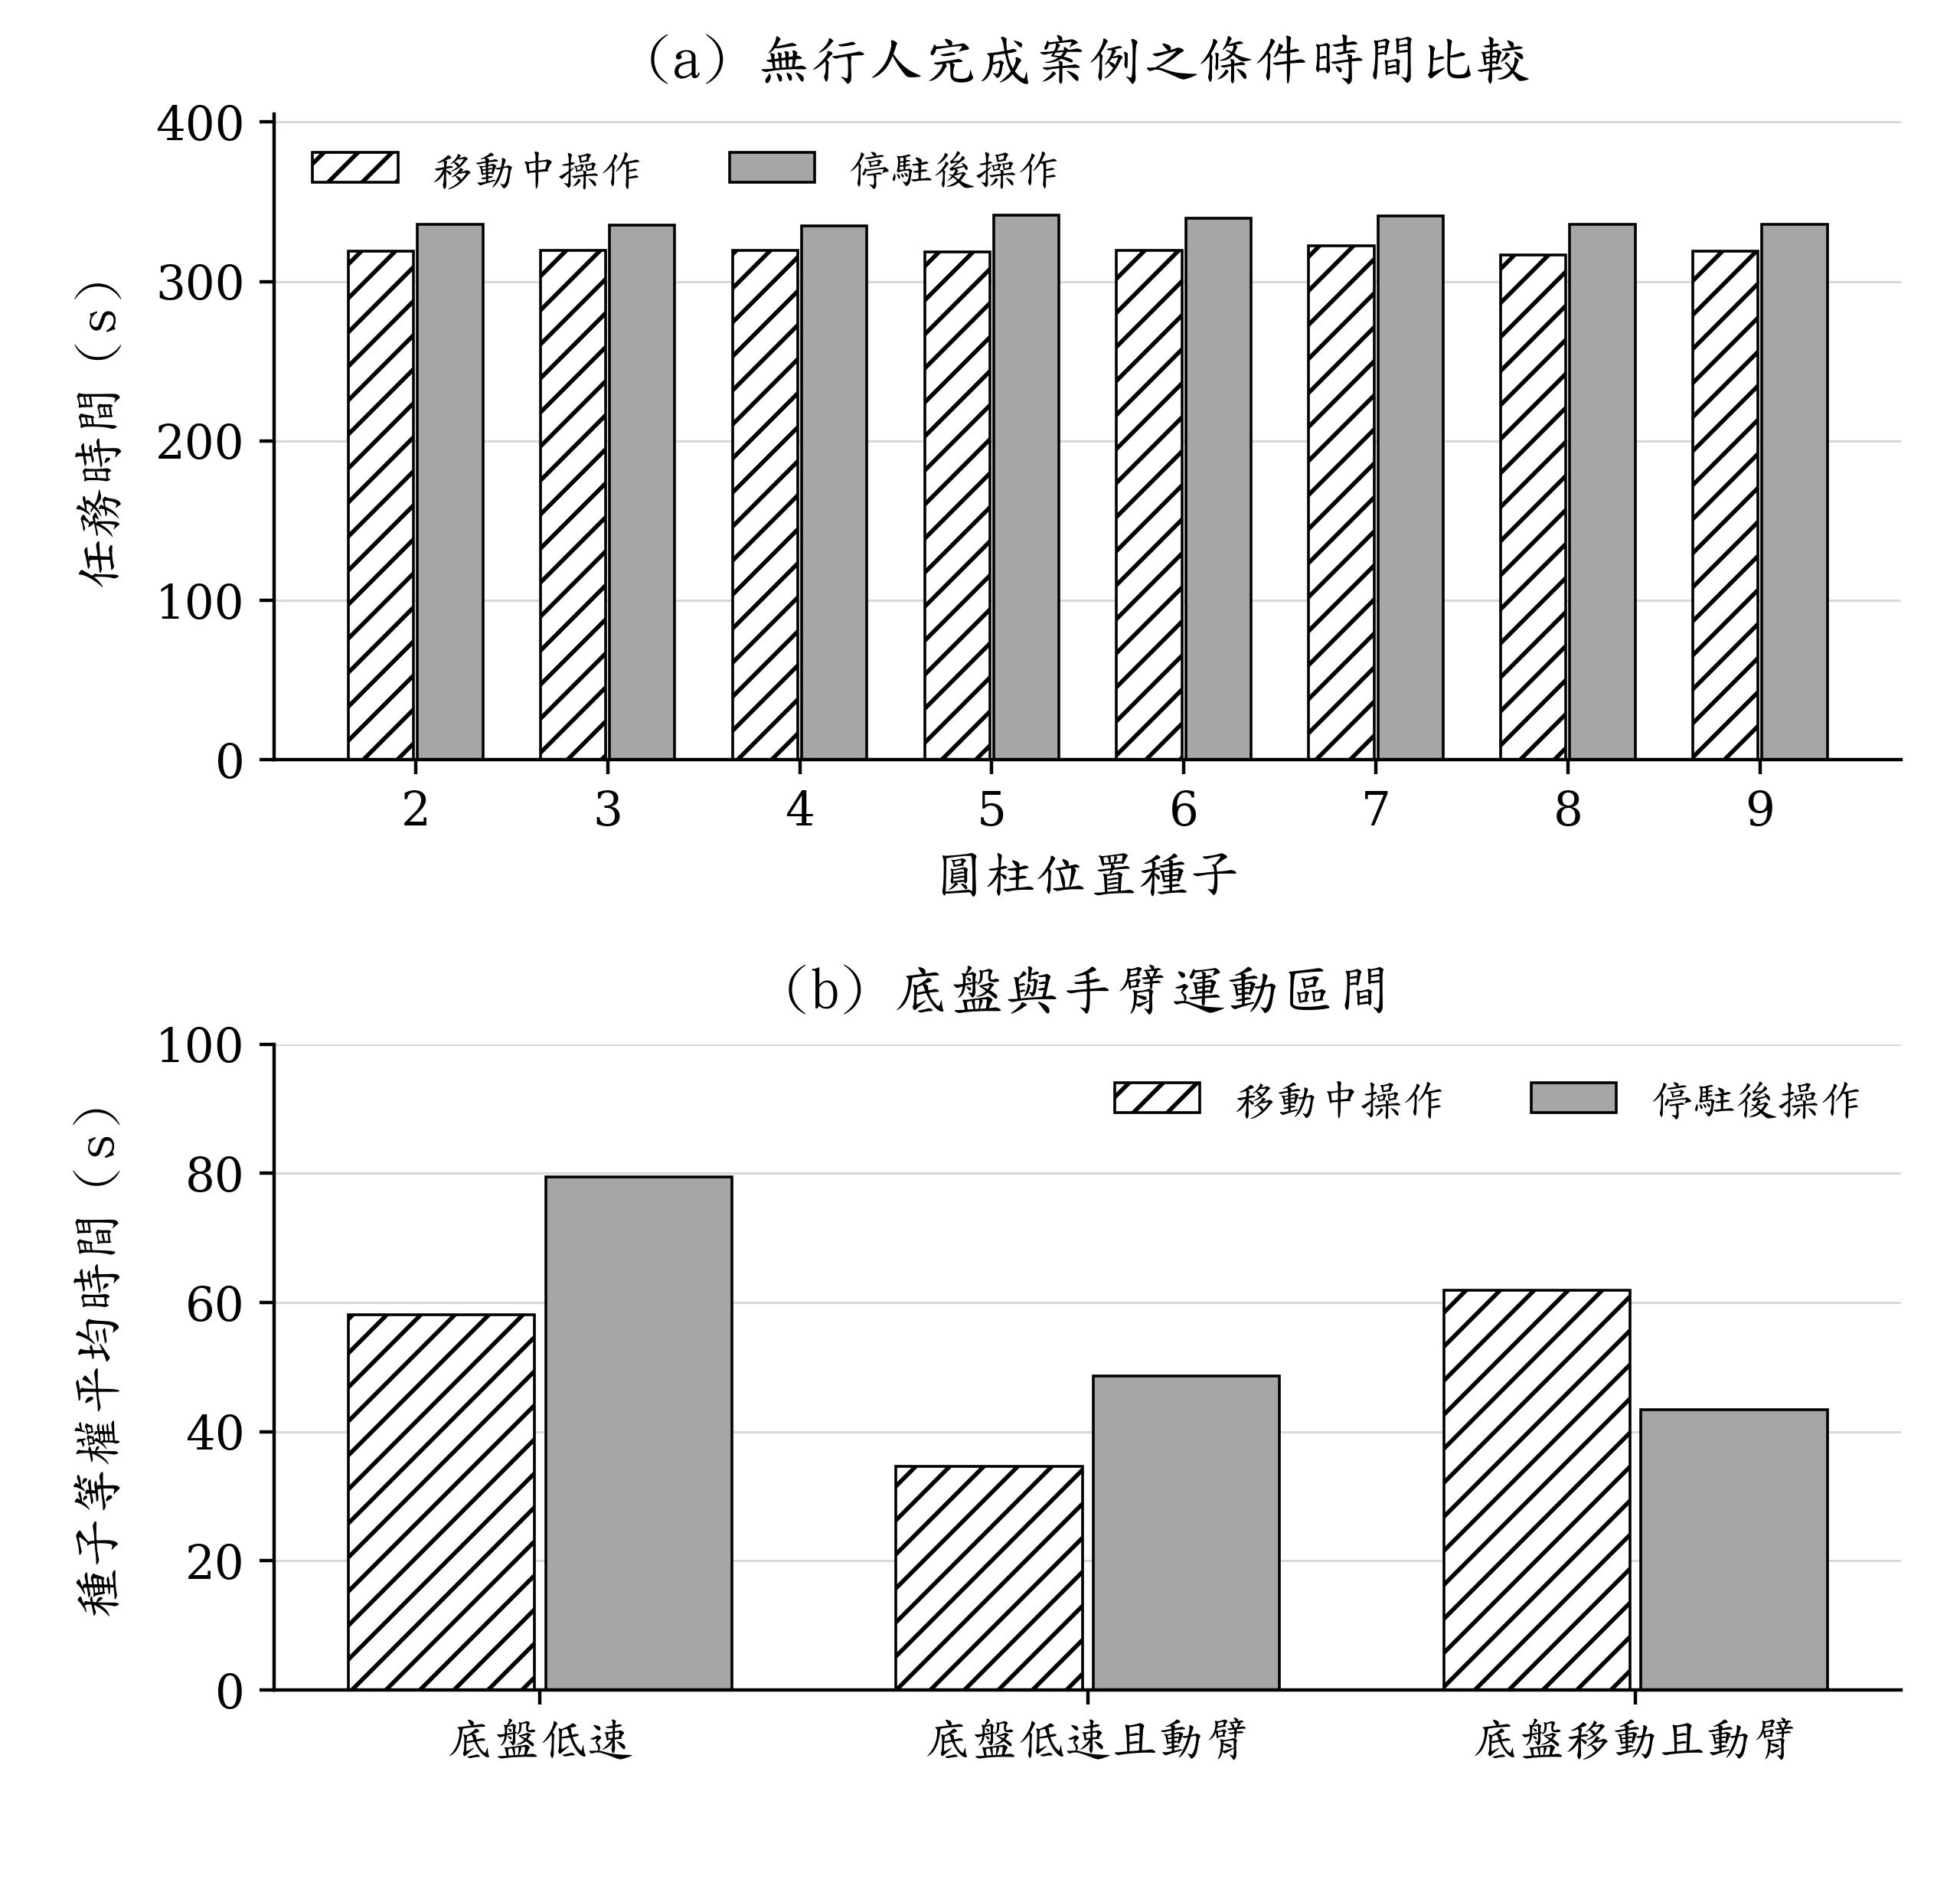
\includegraphics[width=0.98\textwidth]{figsrc/ch04/residential_strategy_seed_comparison.png}
    \caption{無行人住宅任務之完成案例比較：
    (a) 八個圓柱位置種子下的任務時間；
    (b) 底盤低速、低速且動臂及移動且動臂的種子等權平均時間。
    同一種子與策略的重複完成紀錄先取平均；
    低速且動臂為低速區間的子集合，各類時間不相加為任務總時間。}
    \label{fig:ch4_residential_strategy_comparison}
\end{figure}

運動重疊區間由 $50$ ms 取樣的位姿與關節差分判定。
底盤低速條件為平移速率小於 $0.01$ m/s 且偏航速率小於 $0.02$ rad/s；
動臂條件為六軸關節速度向量範數大於 $0.05$ rad/s；
底盤移動且動臂另要求平移速率大於 $0.03$ m/s。
依此定義，移動策略的平均底盤低速時間由 $79.39$ 降至 $58.14$ s，
低速且動臂時間由 $48.60$ 降至 $34.61$ s，
移動且動臂時間則由 $43.44$ 增至 $61.90$ s，
如\cref{fig:ch4_residential_strategy_comparison}(b)所示。
這些結果呈現接近與手臂運動重疊對任務時間安排的影響，
其追蹤品質、計算期限及中止原因仍需配合個別紀錄分析。
